\graphicspath{{02-TOF/Figures/}}


\newcommand{\mchange}[2]{{\color{red}#1}{\color{green}#2}}
\newcommand{\malert}[1]{{\it\color{red}#1}}
\newcommand{\hilite}[1]{{\it\color{blue}#1}}
\newcommand{\Tzero}{\ensuremath{T0}}
\newcommand{\Gauss}{\ensuremath{\text{G}}}
\newcommand{\DT}{\ensuremath{\Delta T}}
\newcommand{\us}{\ensuremath{\mu\text{s}}}

\section{Time-of-Flight Detectors}
\label{Sect:TOF}

% List of figures
% \begin{itemize}
% \item PMT charge correlation PMT0 vs PMT1 - maybe, if relevant
% \item \hilite{TW calibration of one channel}
% \item \hilite{Slab DT before TW correction and after - single pixel.}
% \item \hilite{Residual TW}
% \item T0 correction for 1 channel - electron peak fit
% \item \malert{(?)} Slab DT mean and sigma for all pixels after
%   calibration
%   \begin{itemize} \it
%   \item depends on whether we are comfortable with showing it
%   \end{itemize}
% \item \hilite{Overall slab DT}
% \item Space-point creation efficiency per pixel/slab
%   \begin{itemize}\it
%   \item this is tricky, the only inefficiency comes from time mismatch
%   \item it can point to a fact that some slabs/pixels have something
%     wrong with them
%   \item it is not measure of performance per se
%   \end{itemize}
% \item Particle detection efficiency
%   \begin{itemize} \it
%   \item don't know how to extract from the data, ideally pixel map for
%     each TOF
%   \end{itemize}

% \end{itemize}


% \malert{Issues:}
% \begin{itemize}
% \item should we use word ``counter'' or ``slab''?
% \end{itemize}

%%%%%%%%%%%%%%%%%%%%%%%%%%%%%%%%%%%%%%%%%%%%%%%%%%%%%%%%%%%%%%%%%%%%%%%%%%%%%%%%
\subsection{Introduction}
\label{SubSect:TOF_Intro}
% version 0.1 edited by Maurizio Bonesini 19/2/2018
% version 0.2 edited 23/10/2018

Three time-of-flight detectors (TOF0, TOF1, TOF2) were built and
installed at RAL in 2008 and 2009 to measure the position and the time
of crossing particles.  TOF0 and
TOF1~\cite{NOTE145},~\cite{NOTE241},~\cite{2010NIMPA.615...14B} were
placed upstream of the cooling channel, and TOF2~\cite{NOTE286} was
downstream of the channel, mounted in front of the KL, as shown
in~Fig.~\ref{fig:BL}.  The time of flight between two TOF stations
provides particle identification information and can also be used for
momentum measurement. TOF1 served most of the time also as an
experimental trigger. They operated smoothly during the so-called
Step~I and Step~IV~\cite{Rajaram:2015bra},~\cite{2015ehep.confE.521B}
running periods of the MICE experiment and were essential for all the
measurements done.

\begin{figure}[!ht]
  \begin{center}
    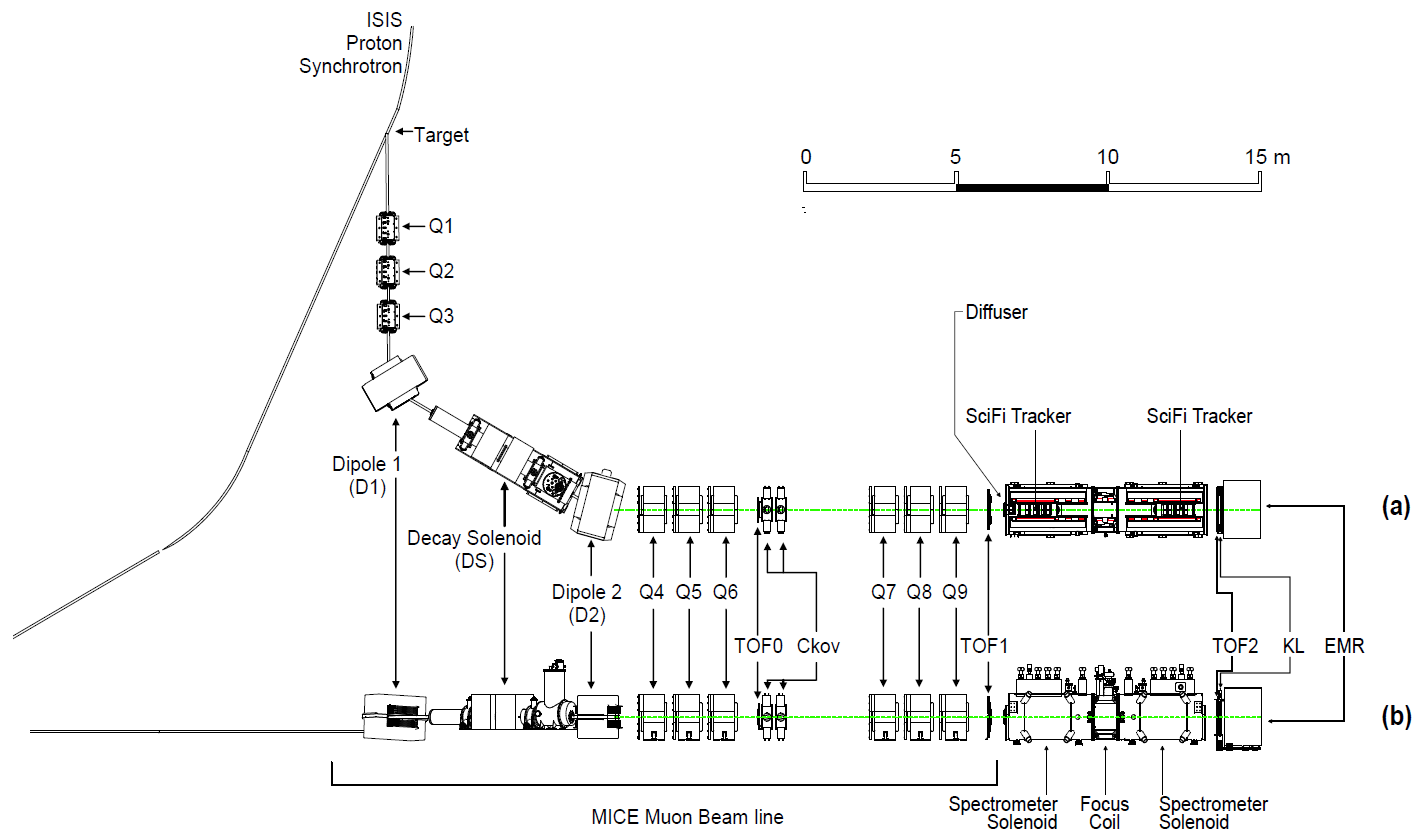
\includegraphics[width=0.8\columnwidth]{BL.png}
    \caption{MICE experiment in the Step~IV configuration, showing the full beam line and cooling channel elements with all the detectors.}
    \label{fig:BL}
  \end{center}
\end{figure}

The good performances of the TOF detectors, over an extended period of time,
enabled the MICE experiment to characterize fully its muon beams during
Step~I data-taking, by measuring their emittance~\cite{2013arXiv1306.1509T} and
assessing their pion contamination~\cite{2016JInst..11P3001A}.

Each TOF station was made of two planes of fast~1''~thick scintillator
bars oriented along X and Y directions, respectively. The bars were
made of BC404 plastic scintillator\footnote{Emission maximum at
  $408$~nm, decay time $1.8$~ns, attenuation length $160~cm$}. A
simple fishtail light-guide was used to attach each end of a bar to
R4998 Hamamatsu fast photomultiplier tubes\footnote{one-inch linear
  focused PMTs with 10 stages, typical gain G$\sim$5.7$\times$10$^6$
  at -2250~V and B=0~T, rise time 0.7~ns, transit time spread
  (TTS)~$\sim$160~ps}.  R4998 PMTs were delivered by Hamamatsu in
assemblies (H6533MOD) that included the PMT tube, the voltage divider
chain and a 1~mm thick $\mu$-metal shield, extending 30~mm beyond the
photocathode surface.  To increase the count rate stability active
dividers were used, instead of conventional resistive
ones. Illustration of TOF1 station is shown in
Figure~\ref{fig:tof:schematic} together with an exploded view of a
slab.

\begin{figure}[!ht]
  \centering
  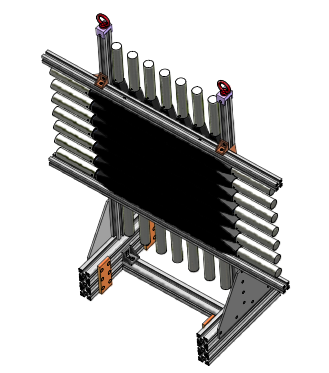
\includegraphics[width=5cm]{tof_diagram}
  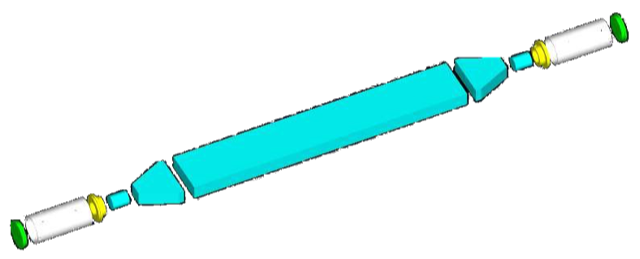
\includegraphics[width=5cm]{slab_design}
  \caption{TOF design~\cite{Rayner:2011zz} and slab components~\cite{NOTE241}.}
  \label{fig:tof:schematic}
\end{figure}

The stations TOF0, TOF1, and TOF2 had active areas of
40$\times$40~cm$^2$, 42$\times$42~cm$^2$, and 60$\times$60~cm$^2$
respectively.  Each of the planes in TOF0 station had 10 4-cm wide
scintillator slabs. Stations TOF1 and TOF2 used 7 and
10 in each plane, respectively.
The PMTs are connected to a $50\%-50\%$ passive splitter using
$\sim$34~m long RG213 signal cable. One half of the signal is fed to
the leading-edge CAMAC Lecroy 4115 discriminator followed by CAEN
V1290 TDC for time measurements. Second half of the signal goes to
CAEN V1724 FADC for pulse-height measurements. Pulse height
measurement is instrumental for time-walk corrections. Each station
issued a local readout trigger if signals in both PMTs attached to a
slab crossed a specific threshold. All three stations were read out when
TOF1 station issued a local trigger. This readout trigger was also
used for the rest of the MICE detector systems.

% Pulse heights and times of the signals
% were recorded if

%\malert{Do we want to include this?:}
% As reported in
%reference~\cite{NOTE241}, RG213 cables\footnote{CERN type C-50-6-1,
%  with rated delay 4.08 ns/m} have a better temperature stability than
%conventional RG58 cables.

% \malert{Unnecessary: Their delay have been individually measured
% in laboratory, before installation in the experimental hall.  Time
% calibration of individual counters has been done with impinging beam
% particles by using the detector X/Y
% redundancy~\cite{NOTE251}. }

All stations were exposed to residual magnetic fields: TOF0 station was placed in a relatively low residual field produced by the last quadrupole magnet of the beam line, while the other two TOF stations were exposed to the stray fields of the cooling channel solenoids. A shielding structure was adopted covering all PMTs at each side of the stations. Fig.~\ref{fig:TOF2} shows photographs from the assembly of the TOF2 station at INFN MIB, taken from \cite{NOTE286}.

%All three stations were exposed to residual magnetic fields. TOF0 station
%was placed in a relatively low residual field ($\le 50~\Gauss$)
%produced by the last quadrupole magnet of the beam line.  The PMTs in
%this station used 1-mm thick $\mu$-metal shielding \malert{(we don't
%  seem to have any reference)}. The other two TOF stations (TOF1/TOF2)
%were exposed to the stray fields of the cooling channel solenoids that
%were only partially shielded by 100~mm thick annular iron plates
%\malert{(need to have a reference, possibly described earlier in the
%  paper)}. The residual magnetic fields were up to 0.13~T (with a
%component along the PMTs axis up to 0.04~T). Box-shaped soft iron
%shielding is more effective than cylindrical one.

% too much about the shielding, removed.
%This idea, pioneered in the D0 experiment \malert{(citation needed, or remove altogether)}, has been
%tested in the case of MICE using different geometrical configurations
%of the iron shielding boxes and different iron materials (e.g. Fe360,
%ARMCO\footnote{ARMCO steel from AkSteel is a pure iron with a maximal
%  carbon content of $0.025\%$ and very high magnetic
%  saturation},~etc) \cite{2012NIMPA.693..130B}.
% Systematic studies were
% performed~\cite{2012NIMPA.693..130B} and
%A composite structure of the shielding was adopted. The first layer of
%the shielding consisted of 1~mm $\mu$-metal around the Hamamatsu
%H6533Mod assemblies. The second layer was an additional box-shaped
%ARMCO bulk with a borehole of 3.2~cm in diameter~\cite{NOTE455} for
%each PMT. A single-bar-like structure was used to shield all PMTs at
%each side of the station. The bars were 15~cm deep, and 5.7~cm or
%6.6~cm thick for TOF1 or TOF2, respectively.  \malert{(Original text
%  stated 6$\times$6~cm$^2$ anfd 5.6$\times$5.6~cm$^2$, 15~cm
%  long. This is with contradiction with the design drawings in MICE
%  note 455 (TOF1) and the drawing provided in this paper (TOF2))}
%Fig.~\ref{fig:TOF1} shows the design drawing of the shielding at the
%TOF2 station detailing individual parts. There was an extra shielding
%effect due to the fact that all bars of the TOF2 PMTs were
%magnetically linked together and also linked to both the KL shielding
%and the shielding plate \malert{(which shielding plate)} making a
%single magnetic loop.
%\begin{figure}
%  \begin{center}
%  \includegraphics[width=9cm,angle=-90]{./02-TOF/Figures/TOF2.eps} \\
%  \caption{Exploded view of the TOF2 detector magnetic shielding for
%    one row of PMTs. Visible are different pieces of ARMCO shielding
%    and the plastic holder and end-caps (left) for mounting the bases of
%    individual PMTs.}
%  \label{fig:TOF1}
%  \end{center}
%\end{figure}

\begin{figure}
  \begin{center}
  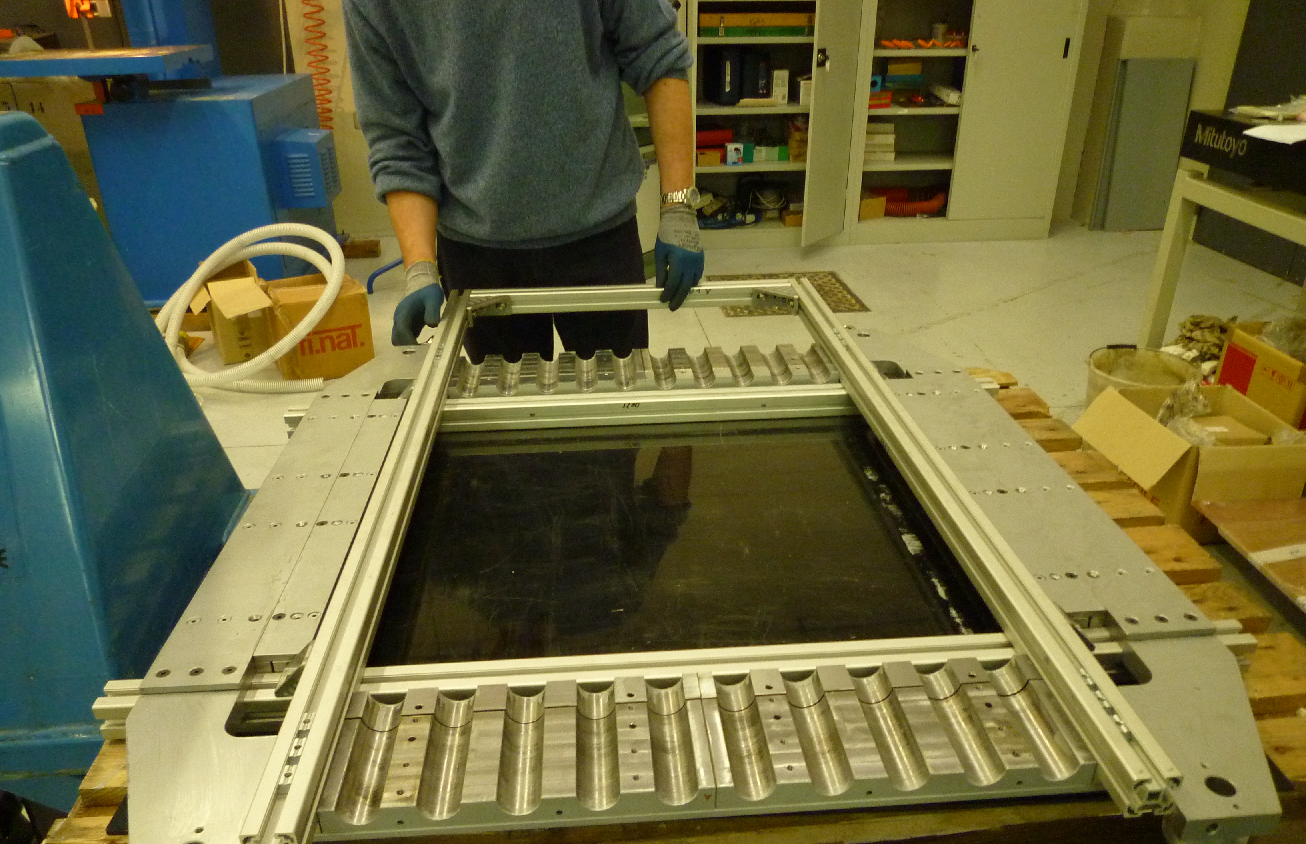
\includegraphics[width=0.24\columnwidth]{./02-TOF/Figures/TOF_assembly_a.png}
  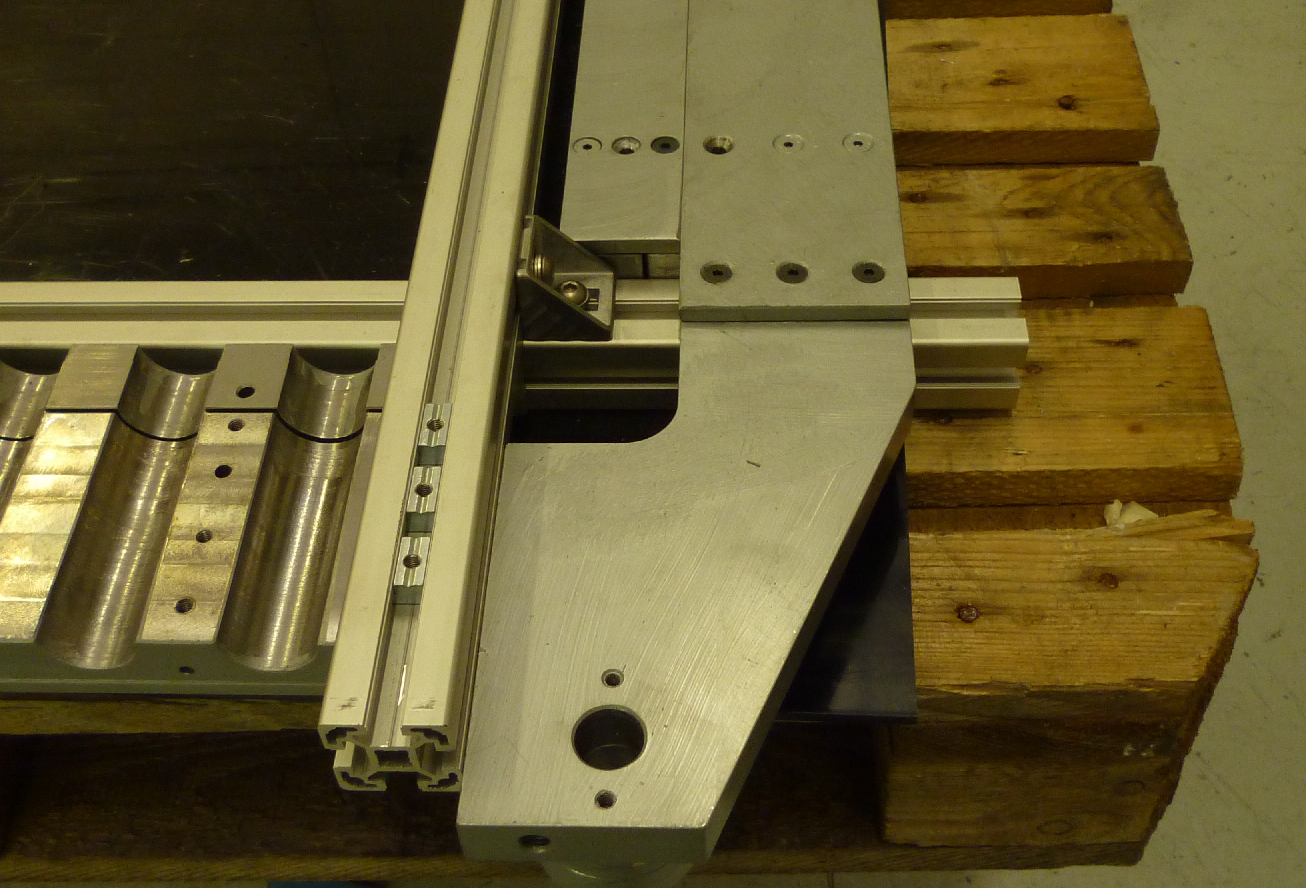
\includegraphics[width=0.24\columnwidth]{./02-TOF/Figures/TOF_assembly_b.png}
  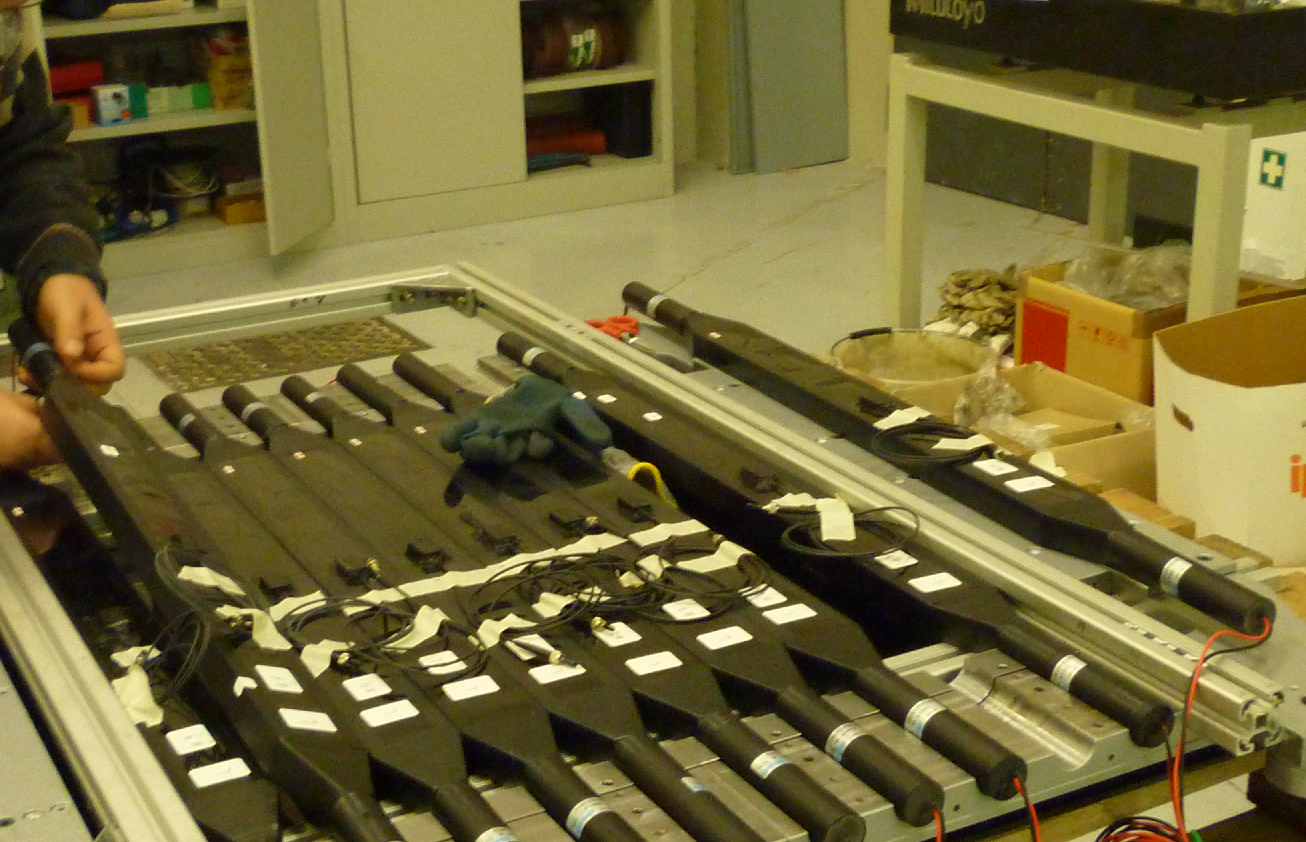
\includegraphics[width=0.24\columnwidth]{./02-TOF/Figures/TOF_assembly_c.png}
  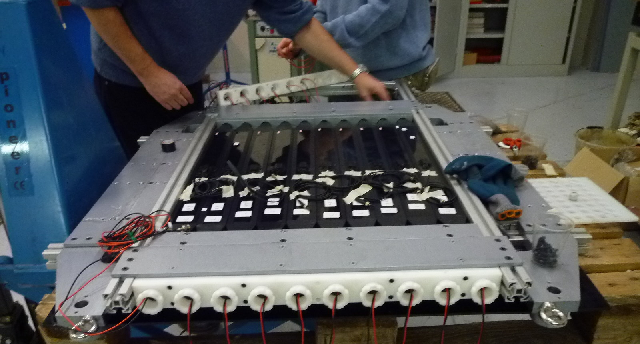
\includegraphics[width=0.24\columnwidth]{./02-TOF/Figures/TOF_assembly_d.png}
  \caption{Assembly of TOF2 at INFN MIB mechanics workshop. Left to
    right: from the bare magnetic shielding to the fully assembled
    counters of one plane.}
  \label{fig:TOF2}
  \end{center}
\end{figure}


% \malert{The following paragraph is summarising the performance. It
%   states overly optimistic performance.}
% \malert{reformulate ---} For what attains performances\malert{---},
% TOF0, TOF1, and TOF2 had timing resolutions around 50-60 ps
% respectively \malert{(currently observed $\sim$110~ps)}, over the 8
% years running period, consistent with design requirements, with the
% spatial resolution around 1~cm. \malert{We don't use any special
%   reconstruction method. Resolution kept at 4 cm or 6 cm for TOF0 or
%   TOF1 and TOF2 respectively. Do we say resolution = 1/2 of strip
%   width or $1/\sqrt{12}$?}  Fig.~\ref{fig:TOF3}~shows distributions of
% the time of flight between TOF0 and TOF1 where electrons, muons and
% pions fall into three well defined peaks.
% \begin{figure}
%   \begin{center}
%     \includegraphics[width=8cm]{./02-TOF/Figures/TOF.png}
%     \caption{Time of flight between TOF0 and TOF1 for a ``pion''
%       beam. From the left: the well separated electron, muon and pion
%       peaks.}
%     \label{fig:TOF3}
%   \end{center}
% \end{figure}


% \malert{What is currently the main purpose of TOFs? This determines
%   the requirements on the performance. Will need to tell that current
%   T-o-F measurement has sufficient resolution, which appears to be
%   $\sim$100-120~ps}

The purpose of the TOF system is to effectively discriminate particle species
based on time-of-flight measurement. The main components in the
MICE beam are muons, pions, and electrons. The time resolution needs
to be sufficiently good to effectively discriminate between these
types. At 240~MeV/c, the time-of-flight difference between muon and
pion is about 1.3~ns between TOF0 and TOF1 stations. With 200~ps
resolution, one reaches near $100\%$ discrimination efficiency.


%%%%%%%%%%%%%%%%%%%%%%%%%%%%%%%%%%%%%%%%%%%%%%%%%%%%%%%%%%%%%%%%%%%%%%%%%%%%%%%%
%The following text describes the method used to calibrate the TOF system and its performance.

\subsection{Calibration Method}
% \begin{itemize}
% \item Describe the method. Based on MICE note 251.
% \item \malert{TOF NIMA paper says that measured time resolution of the
%     CAEN TDC was 22~ps/count, as opposed  to declared 25~ps!}
% \item  Some description of the calibration method is also described in the
%   paper.
% \item  \malert{There's a short description of the method also in Rayner's
%     Thesis, Section 3.2.1 and Appendix B (this is improved method to
%     extract more calibration constants for proper x,y measurements,
%     Rayner claims $\sim$1~cm resolution; our current resolution = slab
%     width / sqrt(12) $\sim 1.2 - 1.7$ ).}
% \end{itemize}

Measurement of time traversal of a particle through a TOF station is
influenced by several factors at the hardware level. When a particle
crosses the plastic scintillator, there is a short delay in light
production, with a characteristic decay time of $1.8~ns$.

After generation, scintillation light propagates to the ends of each
scintillator slab where it is detected by photomultiplier tubes. The
light-travel time depends on the distance of the particle crossing
from the PMT. The lengths of slabs in TOF0, TOF1, and TOF2 were 40~cm,
42~cm, and 60~cm, respectively. This translates to about 3~ns, 3.1~ns,
and 4.4~ns, respectively, as the effective light propagation speed in
the scintillator was found to be approximately 13.5~cm/ns.

More delay was introduced by the transit time of each PMT and of the
cable that led the signal to the readout electronics. These times were
unique for each individual PMT channel and needed to be determined in
dedicated measurements.

The times of each signal of a PMT were measured as times of signal threshold
crossings in a simple linear discriminator. This introduced bias in
the measured time dependent on the total charge of the signal, effect
referred to as time-walk.

Signal times of each channel were recorded in TDC boards. Readout of
the whole system was triggered by having a signal in TOF1 station. The
readout trigger signal is distributed to all TDC boards and is used as
a reference time. Which PMT channel's threshold crossing caused the
readout was depending on where the particle crossed through the TOF1
station. As a consequence, the reference time had a bias dependent on
the position of TOF1 crossing, an effect referred to here as trigger
delay.

The final time measurement in each station was determined as an average of
the times of individual channels. This way, different distance from
the point of crossing to each side of the scintillator slabs does not
matter anymore, because the average of the times of the 2 PMTs does
not depend on it.

Corrections which need to be made to the measured times are then the
time-walk correction, the PMT channel specific delay time $T0$, and
a correction for the reference trigger time delay.

Details of the calibration method are described in \cite{NOTE251}.


%%%%%%%%%%%%%%%%%%%%%%%%%%%%%%%%%%%%%%%%%%%%%%%%%%%%%%%%%%%%%%%%%%%%%%%%%%%%%%%%
\subsubsection{Time-walk Correction}
% \begin{itemize}
% \item  \malert{Fig of a selected PMT TW 2D hist. + Profile + Fit}
% \item  \malert{Fig of residual TW.}
% \item  \malert{Fig of Slab DT before TW
%     correction and after.}
% \end{itemize}

First correction to the measured time of each channel is time-walk
correction. It was considered to be a static property of each
channel. The same correction was used for all runs. The correction was
determined by looking at time difference between two selected channels
of slabs from different planes.

Let $T^{ijk}$ denote a TDC measured time in PMT $k$ of a slab $j$ in a
plane $i$. Similarly, let $ADC^{ijk}$ be the measured pulse height in
that PMT channel. Then time-walk of PMT $k$ in slab $j$ of plane 0 was
determined from the 2D distribution of $T^{14k'} - T^{0jk}$
vs.~$ADC^{0jk}$. The reference channel was chosen from slab in the middle
of the other plane (slab 4 in this example). PMT with higher mean ADC
count was selected.

A special pre-correction was first determined for reference slabs,
middle slabs in each plane. Only events where particle crossed the
pixel corresponding to their crossing were considered. The pixel
was in the centre of the station and was always well populated with
particles crossing it.  The ADC count in one of the slabs taken as a
reference was limited to a $10\%$ region around its mean. The TDC time
of the slab was then little affected by the time walk.

The following function was fitted to the profile of the 2D data histogram:
%
\begin{equation}
  \newcommand{\ADC}{\text{ADC}}
  \label{eq:twf}
  f(\ADC) = P_1 + \frac{P_2}{\ADC - P_0} + \frac{P_3}{\left(\ADC - P_0\right)^2}.
\end{equation}
%
Where possible, parameter $P_3$ was fixed to 0. For some PMTs such fit
would not follow the measured trend and the additional parameter was
added to the fit.

After the pre-correction of the reference slabs, time-walk of all the
PMT channels was determined by looking at events in pixels
corresponding to the crossing with the reference slab.

An example of time walk of a channel with respect to pre-corrected
time in a reference slab is shown in Figure~\ref{fig:TW}. The residual
effect of time walk after the correction is also shown.

\begin{figure}
  \begin{center}
  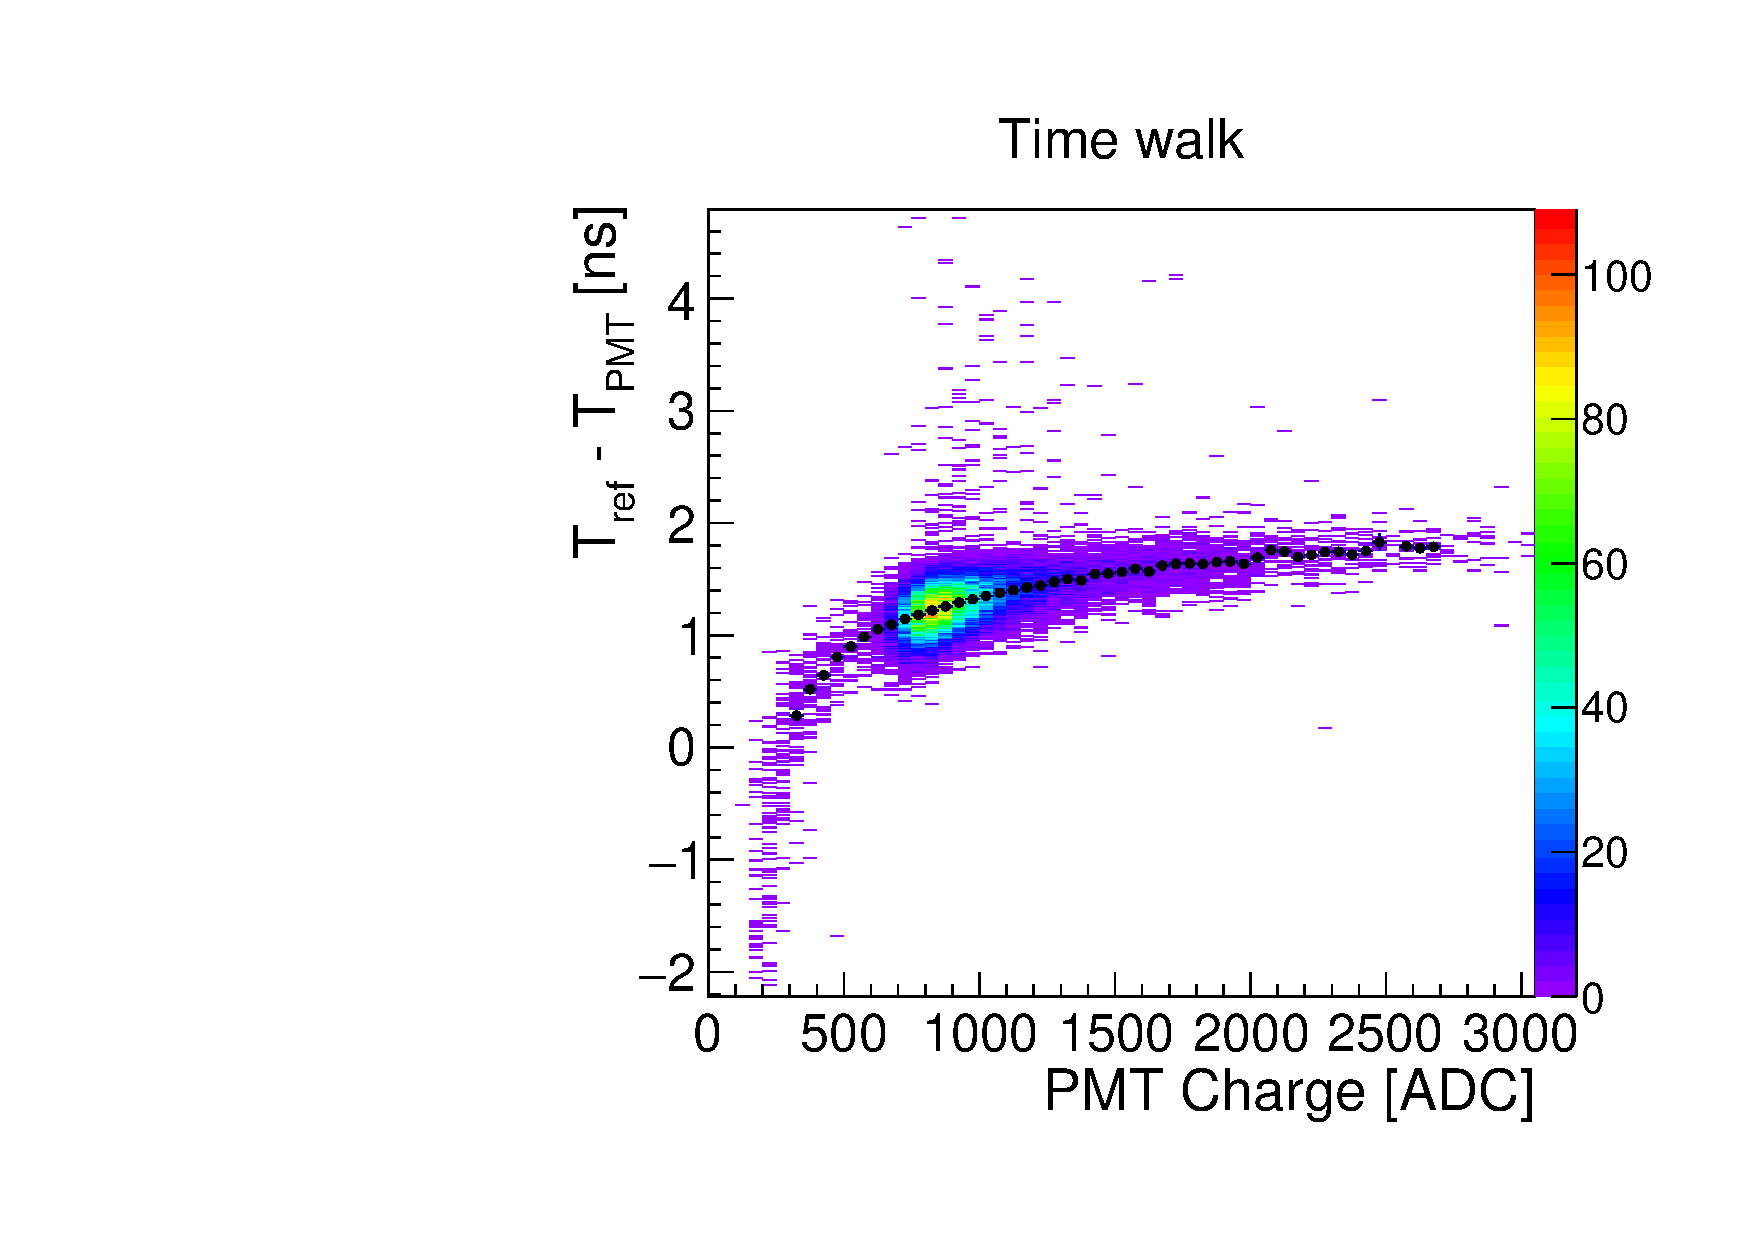
\includegraphics[width=0.45\columnwidth]{01_tw_example}
  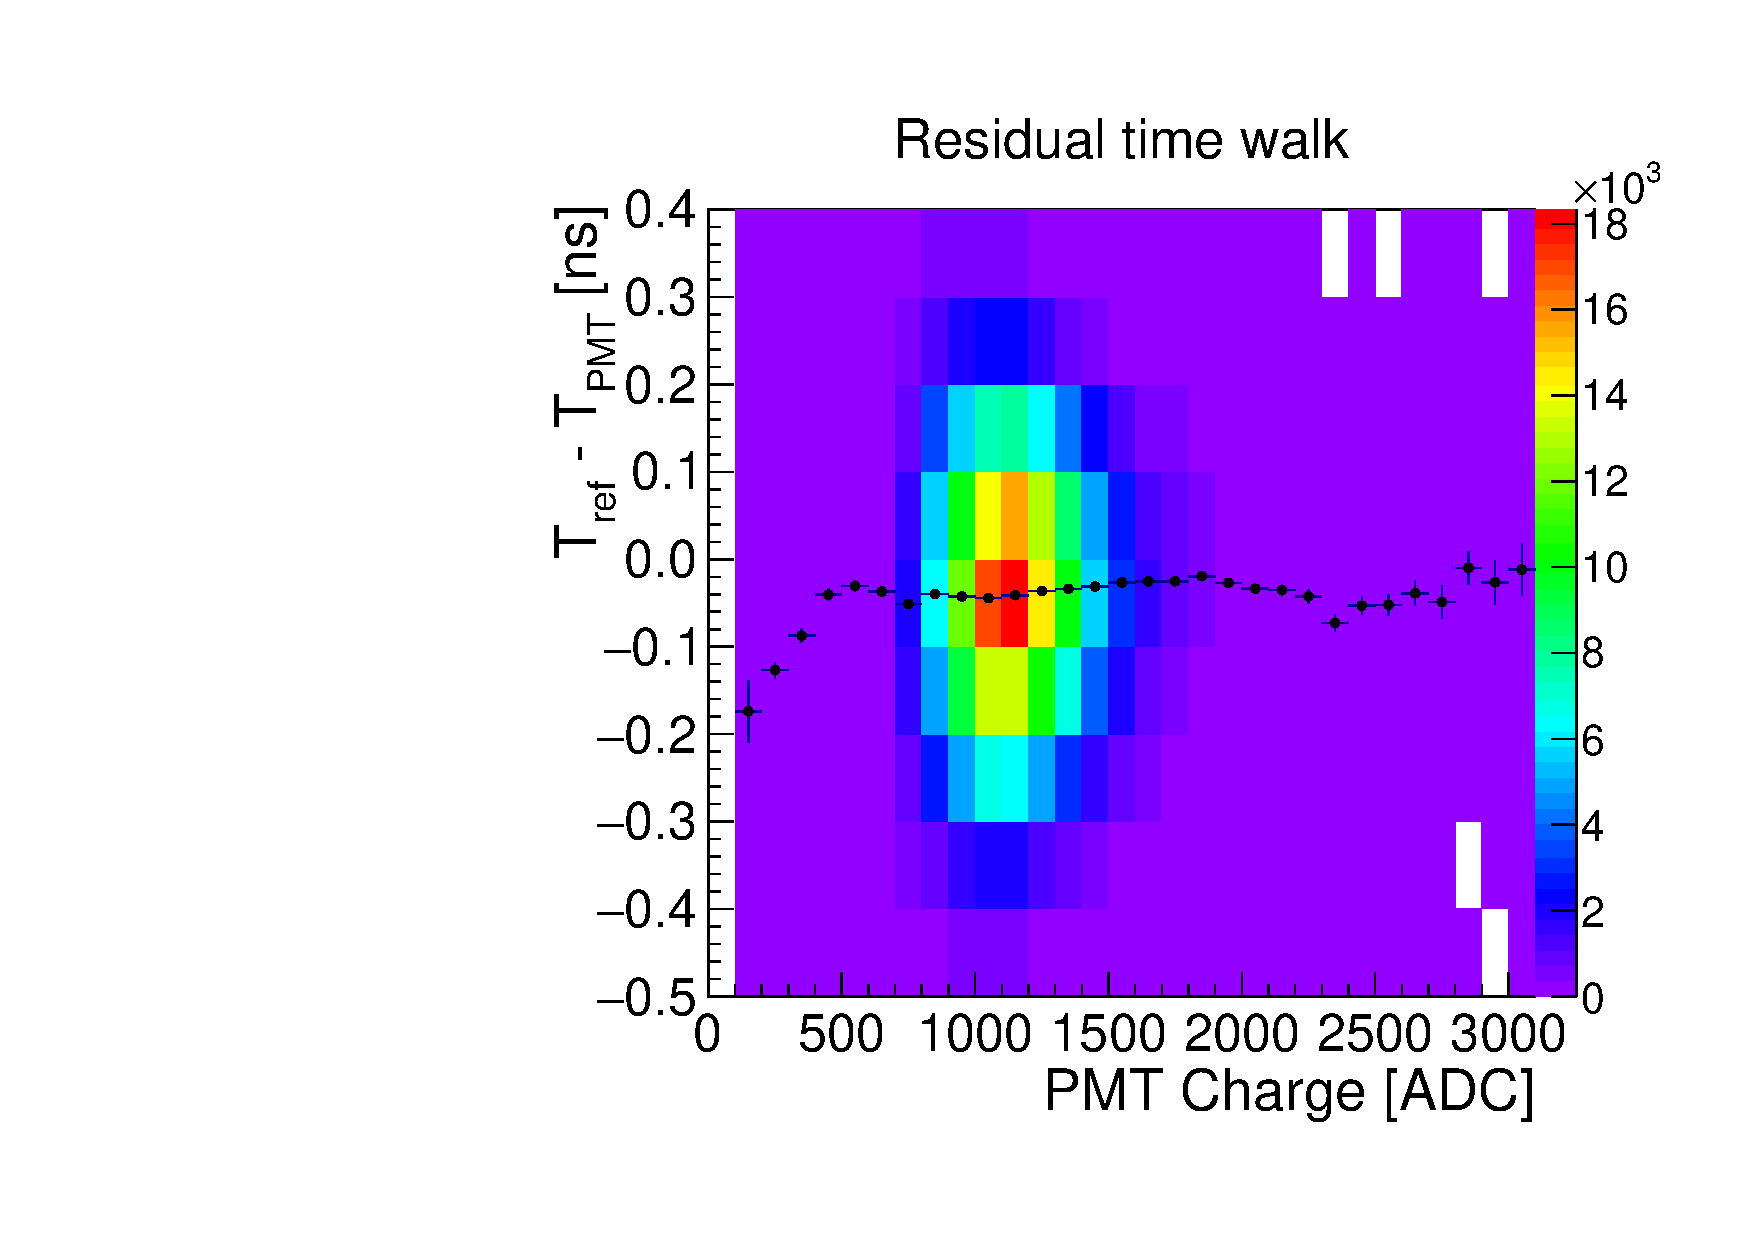
\includegraphics[width=0.45\columnwidth]{03_residual_tw_example} \\
  \caption{Time walk (left) in PMT 0 of slab 4 in plane 0 (horizontal)
    of station TOF0: the 2D histogram (coloured scale) is overlaid
    with its profile and with the fit function described in
    Eq.~\ref{eq:twf}. Residual time walk (right) after the
    correction was applied.  }
  \label{fig:TW}
  \end{center}
\end{figure}



Figure~\ref{fig:SlabDTTW} shows distributions of time differences
between horizontal slab 4 and vertical slab 5 before and after the
time-walk correction. The width of the distribution is significantly
decreased. The mean of the distribution is not centered at 0 as
differences in delays \Tzero{} were not accounted for, yet.

\begin{figure}
  \begin{center}
  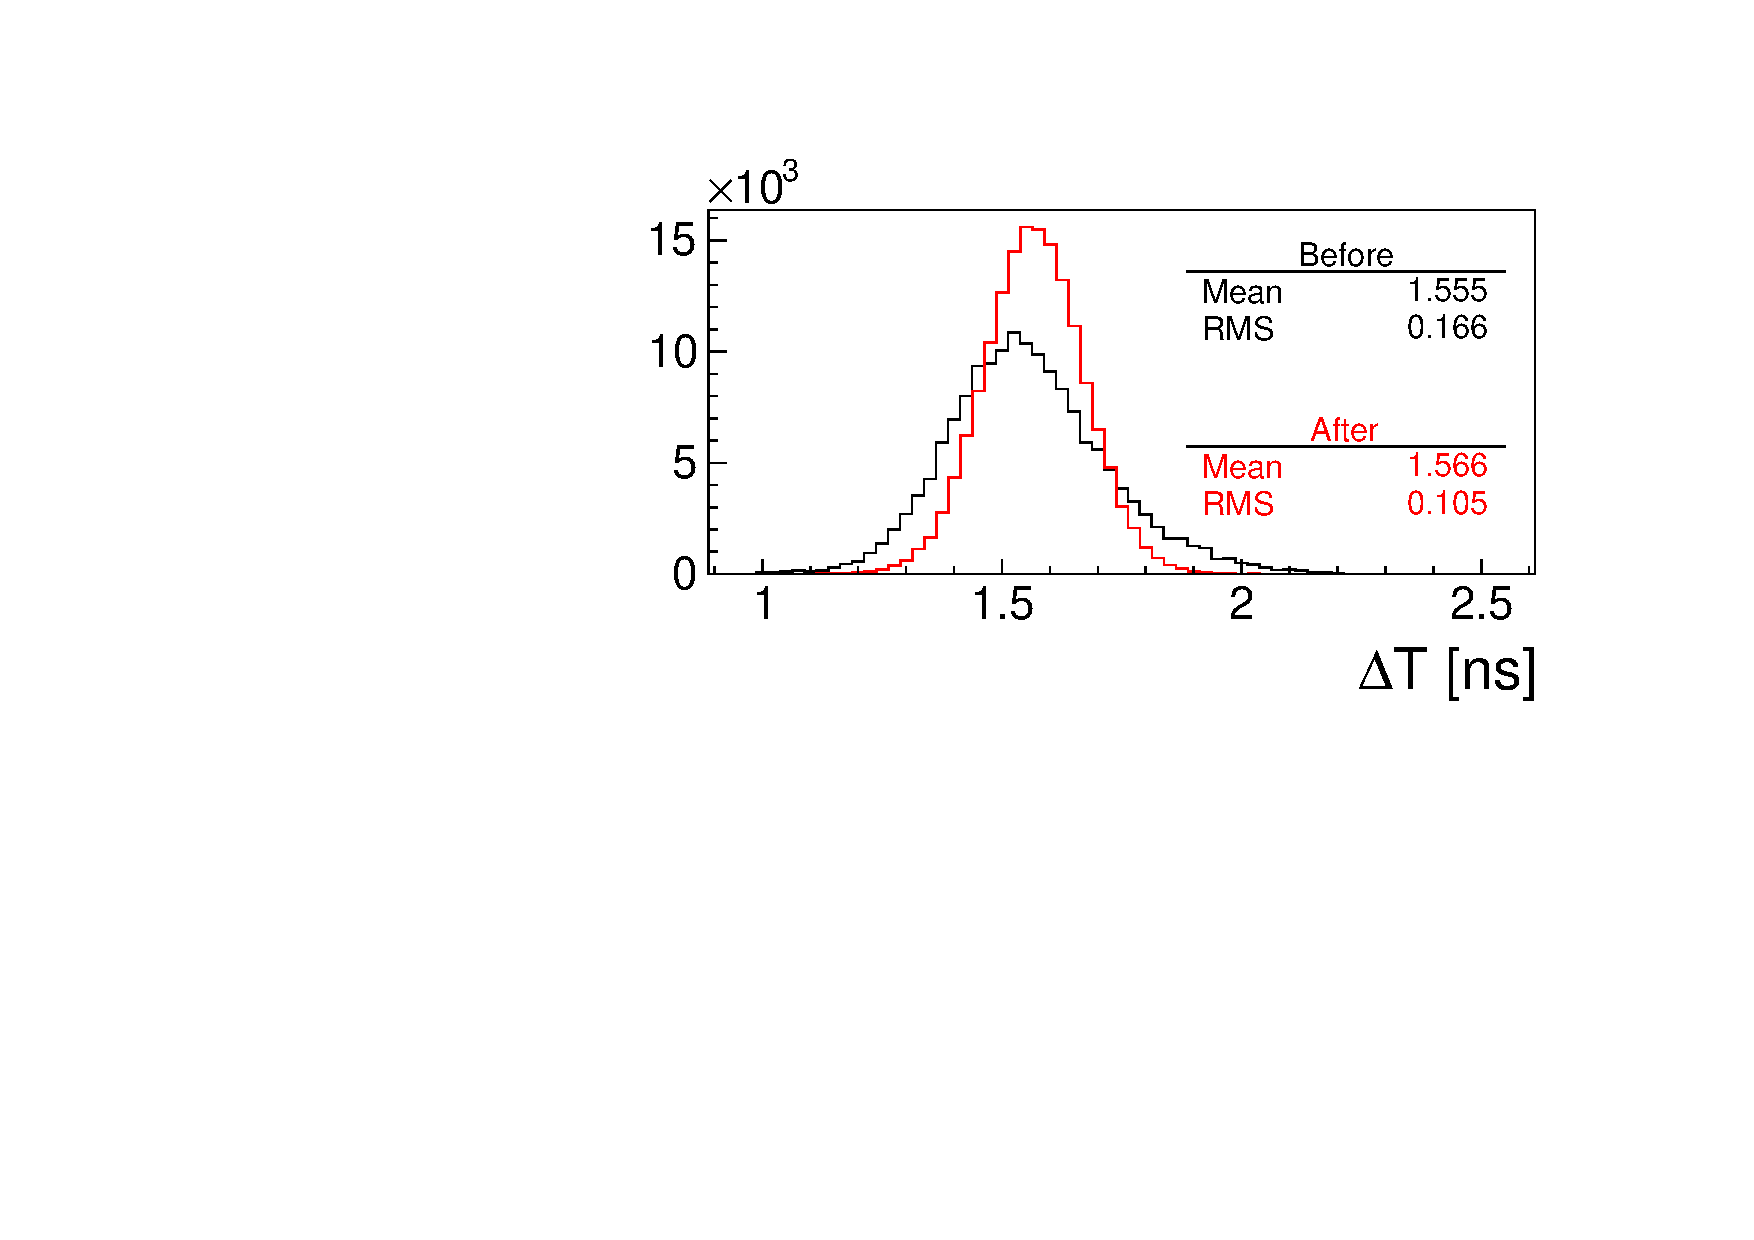
\includegraphics[width=0.5\columnwidth]{02_slab_dt_resolution_tw_effect}
  \caption{Distribution of time differences \DT{} between horizontal slab 4 and
    vertical slab 5 in station TOF0. Distribution before and after the
  time-walk correction are overlaid.}
  \label{fig:SlabDTTW}
  \end{center}
\end{figure}


%%%%%%%%%%%%%%%%%%%%%%%%%%%%%%%%%%%%%%%%%%%%%%%%%%%%%%%%%%%%%%%%%%%%%%%%%%%%%%%%
\subsubsection{Trigger Delay Correction}

\newcommand{\Tdelay}[2]{\ensuremath{T_{\text{tr}}^{#1,#2}}}
\newcommand{\TW}{\ensuremath{\text{TW}}}
\newcommand{\PMT}{\ensuremath{\text{PMT}}}
\newcommand{\ttrig}[2]{\ensuremath{{t}_{#2}^{#1}}}
\newcommand{\mean}[1]{\ensuremath{\left< #1 \right>}}

% Station TOF1 was used to trigger the readout of the whole system. Time
% of it's trigger signal was used as a reference signal to which times
% of each channel of all 3 stations were measured. A two-fold coincidence
% of signals crossing threshold in PMTs on both sides of a slab is
% required.
% %
% For an incoming particle the trigger signal is given by the first of
% the twofold coincidences from slab i and slab k. The time of the
% coincidence signal is the time of the latest signal arriving to the
% logic unit.
% %
% Which PMT channel will be causing trigger depends on the position
% within the slab of the particle crossing and the \Tzero{} delays of
% individual PMTs. Assuming that light arrival time does not change
% significantly across a pixel and no other effects influence signal
% arrival one can expect that passage of a particle through a given
% pixel causes always the same time sequence of PMT signals and the
% delay of the trigger signal will be that of one particular channel in
% each pixel. This assumption, however, does not hold for all
% pixels. The main reason being the time walk effect which biases each
% channel differently and in some pixels results in more than 1 PMT
% channel generating the trigger signal.

Station TOF1 was used to trigger the readout of the whole system. Time
of it's trigger signal was used as a reference signal for time
measurements of all 3 stations. Depending on position where a particle
was crossing the TOF1 station, this trigger signal will have different
delays. The delay of each pixel was measured relative to the central
pixel of TOF1 station. It was assumed that the source of the delay for
individual pixel did not change from event to event. Although in
reality this was not the case for most of the pixels, it was a good
enough approximation.

Determination of the trigger delays for each pixel was as follows:
Times of each PMT were corrected for time walk first. Trigger delay of
the central pixel, defined as a crossing of station's 2 reference
slabs, was set to 0. Trigger delays of the rest of the pixels in the
reference slabs were calculated from differences of mean times of each
PMT. For example, for pixels $i$ of the horizontal reference slab
$\text{refx}$, the trigger delay time $T^\text{trig}_{\text{refx},i}$
is given by:
%
\begin{linenomath}
  \begin{equation}
    \label{eq:trigdel:a}
    T^\text{trig}_{\text{refx},i} =
    \frac12\sum_{\PMT}
    \mean{t^{\PMT, \text{refx}}_{\text{refx},i}} -
    \mean{t^{\PMT,\text{refx}}_{\text{refx},\text{refy}}},
  \end{equation}
\end{linenomath}
%
where $t^{\PMT, i}_{i,j}$ is the time in PMT of slab $i$ for events
where particle crossed pixel $i, j$. The delays are averaged over both
PMTs of the slab. Pixel denoted refx,refy is the central reference
pixel of the TOF1 station.

For the rest of the pixels, not defined by the reference slabs, the
trigger delay times were determined as a delay with respect to the
pixels on the reference slabs. Delays of those reference pixels were
then added:
%
\newcommand{\Ttrig}[1]{\ensuremath{T^\text{trig}_{#1}}}
%
\begin{linenomath}
  \begin{equation}
    \Ttrig{i,j} =
    \frac14\sum_{\PMT}
    \left(
      \mean{\ttrig{\PMT,i}{i,j}} - \mean{\ttrig{\PMT,i}{i,\text{refy}}} +
      \mean{\ttrig{\PMT,j}{i,j}} - \mean{\ttrig{\PMT,j}{\text{refy},j}}
    \right)
    + \frac12
    \left(
      \Ttrig{i,\text{refy}} + \Ttrig{\text{refx},j}
    \right)
    \label{eq:trigdel:both}
  \end{equation}
\end{linenomath}

% Figure~X shows comparison of time-walk corrected times of a particular
% PMT channel for particles passing through two different pixels. The variation
% in position of the peaked distributions is clearly visible.

% Figure~Y shows times measured in a channel in TOF0 station for
% particles crossing the station's central pixel (4,5). Times
% before correction for the trigger signal delay are compared to times
% after the correction.

%%%%%%%%%%%%%%%%%%%%%%%%%%%%%%%%%%%%%%%%%%%%%%%%%%%%%%%%%%%%%%%%%%%%%%%%%%%%%%%%
\subsubsection{$T0$ Correction}

Times in each channel were also corrected for the channel specific
delays caused by each PMT and by the cable lengths. The correction was
determined from times measured of particles crossing through the
middle pixel of each slab. The times were corrected for the time walk
and for TOF0 and TOF2 stations also for the trigger signal delay. The
correction for TOF1, the readout triggering station, were set such
that the mean of the time distribution was at 0.

Times in TOF0 and TOF2 stations reflected the time of flight of
individual particles to and from TOF1. Distribution of the times in
those stations show 3-peaked structure, where the most isolated peak at
lowest time-of-flight corresponds to the electrons. They travel at the
speed of light and their time of flight was calculated from
distances from TOF1 station. Corrections for each channel were
determined such that the electron peak was located at the predicted
time of flight.

Figure~\ref{fig:tof0times} shows position of the electron peak as
measured by TOF0 station in one run with beam at nominal
140~MeV/c. Uncorrected raw times are compared to fully corrected
time. Corrected-time distribution shows better electron peak
separation and it also places it to the correct position relative to
TOF1.

Due to the presence of focusing fields in the beam-line section
between TOF0 and TOF1 stations, particles did not travel in a straight
line in that section. Deviation from a straight line was dependent on
the initial direction and momentum of the particles entering the
section. The effect was estimated~\cite{Rayner:2011zz} in
simulations to be of an order of $\sim$30~ps. This effect caused a
small bias in the calibrations.

\begin{figure}[!ht]
  \centering
  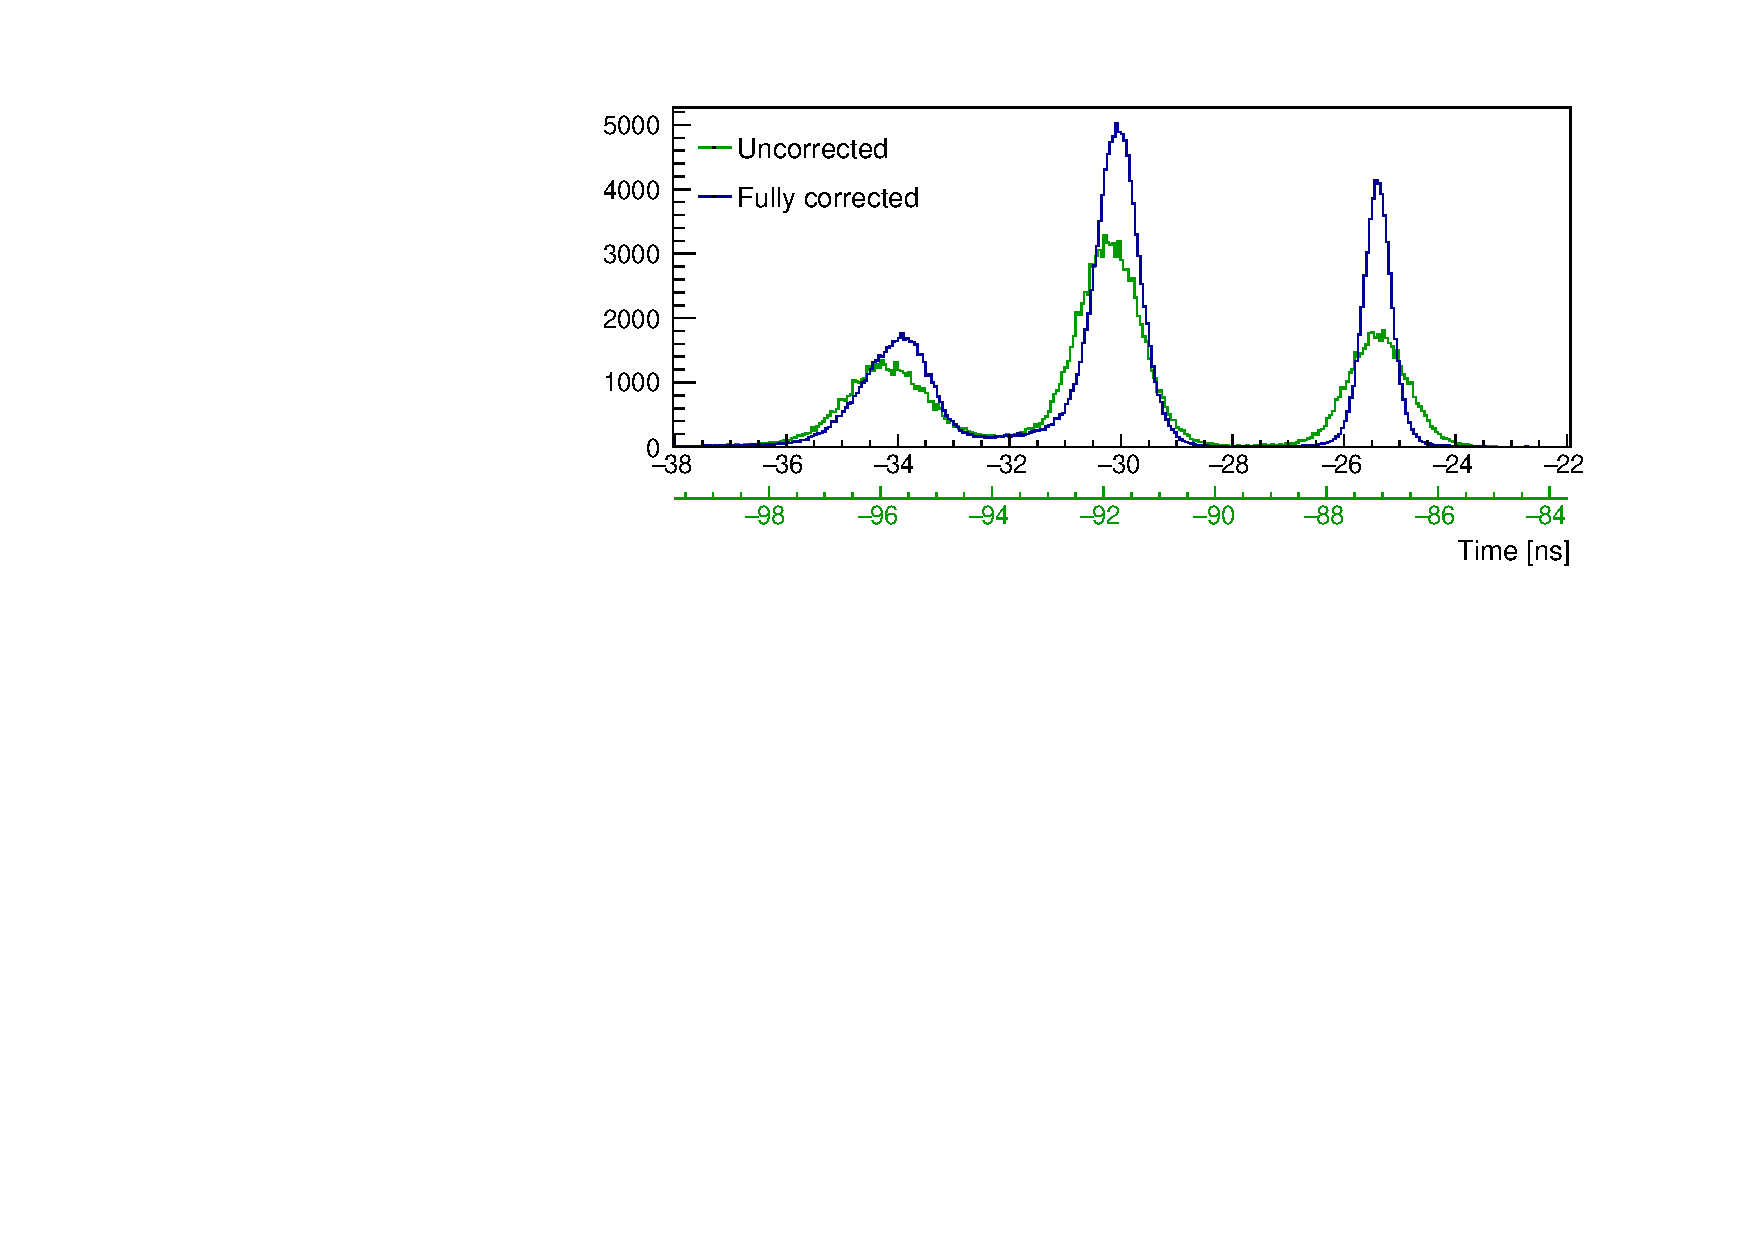
\includegraphics[width=0.8\columnwidth]{04_tof0_corrected_vs_uncorrected}
  \caption{Example of time distribution of events in TOF0. Times
    before any corrections are compared to to times with all
    corrections applied.}
  \label{fig:tof0times}
\end{figure}

%%%%%%%%%%%%%%%%%%%%%%%%%%%%%%%%%%%%%%%%%%%%%%%%%%%%%%%%%%%%%%%%%%%%%%%%%%%%%%%%
\subsection{Reconstruction}

Particle crossing a TOF station must have crossed 2 orthogonal slabs
in the stations 2 planes.  The time and approximate position of
particle crossing a TOF station was reconstructed from the PMT signals
in the two slabs. Each slab with at least one recorded signal in each
of the 2 attached PMTs was considered as being crossed by a
particle. Times of these recorded signals were corrected for
time-walk, readout trigger signal delay, and the channel specific
delay. Time of crossing of the slab was then taken as the average of
the 2 corrected PMT times.

The 2 slabs hit by a particle defined a pixel of area given by the
width of the slabs. Sometimes, there were more slabs in each plane
with signals. Matching of 2 slabs being crossed by a particle was done
based on their measured signal time. They were matched if the times
were within a 4-ns window. The time of the particle crossing was
determined as the average of times of the 2 matched slabs.


In order to be able to correct for the trigger signal delay, the pixel
through which the particle crossed TOF1 needed to be determined. All
possible combinations of 2 slabs from 2 different planes were
tested. The times of the recorded PMT signals were corrected under the
hypothesis that correct slabs were matched. The pixel of the crossing
particle was identified if the time difference of the 2 slabs was
shorter than 4~ns.


%%%%%%%%%%%%%%%%%%%%%%%%%%%%%%%%%%%%%%%%%%%%%%%%%%%%%%%%%%%%%%%%%%%%%%%%%%%%%%%%
\subsection{Performance}
\label{SubSect:TOF_Performance}

% \malert{Several figures are already in the TOF NIMA paper.}



% Figures to show here:
% \begin{itemize}
% \item Slab DT - selected slabs/counters + overall TOFs
% \item ToF10 - + detail of electron peak
%   \begin{itemize} \it
%   \item will need to argue why the peak is broader than stated
%     resolution
%   \item the effect of electron's flight path due to focusing fields is
%     non-negligible - use estimates from Rayner's thesis
%   \end{itemize}
% \item Space-point reconstruction efficiency
%   \begin{itemize}
%   \item shows that slab hits are within the required cut
%     \begin{itemize}
%     \item events with 2 slab hits only
%     \end{itemize}
%   \item inefficiency from:
%     \begin{itemize}
%     \item only single slab hit by different particles in the given
%       spill/bunch
%     \item this may be due to inefficiency of hit creation when
%       particle crosses by the edge of the slab -- see Rayner's
%       thesis/presentations
%     \item two particles share one slab - earlier particle's hit only
%       considered - but this is not considered in these plots (only 2
%       slab hits recorded)
%     \end{itemize}
%   \end{itemize}
% \item Stability of electron peak - run by run position of electron peak!
% \item particle detection efficiency - how to show?
% \item Resolution
%   \begin{itemize}
%   \item Slab DT for all TOFs, show similar performance, although
%     they have different construction.
%   \end{itemize}
% \item \malert{(?)}Efficiency
% \end{itemize}

Resolution of time-of-flight measurement is given by time resolution
of each station. The time of a station particle crossing is determined
from the average of times of the two slabs. The resolution of the
average is a half of the spread of their difference. Therefore,
looking at slab \DT{} allows determination of the time-of-flight
resolution.

Due to the errors in calibrations, especially in the underpopulated
peripheral pixels, the slab \DT{} distributions have slight offsets
from 0. Also, the spread of the distributions varies from pixel to
pixel. The offsets and the spreads of the slab \DT{} distributions for
individual pixels are shown in
Figures~\ref{fig:SlabDToffsetByPixel}~and~\ref{fig:SlabDTresByPixel},
respectively.


\begin{figure}
  \begin{center}
  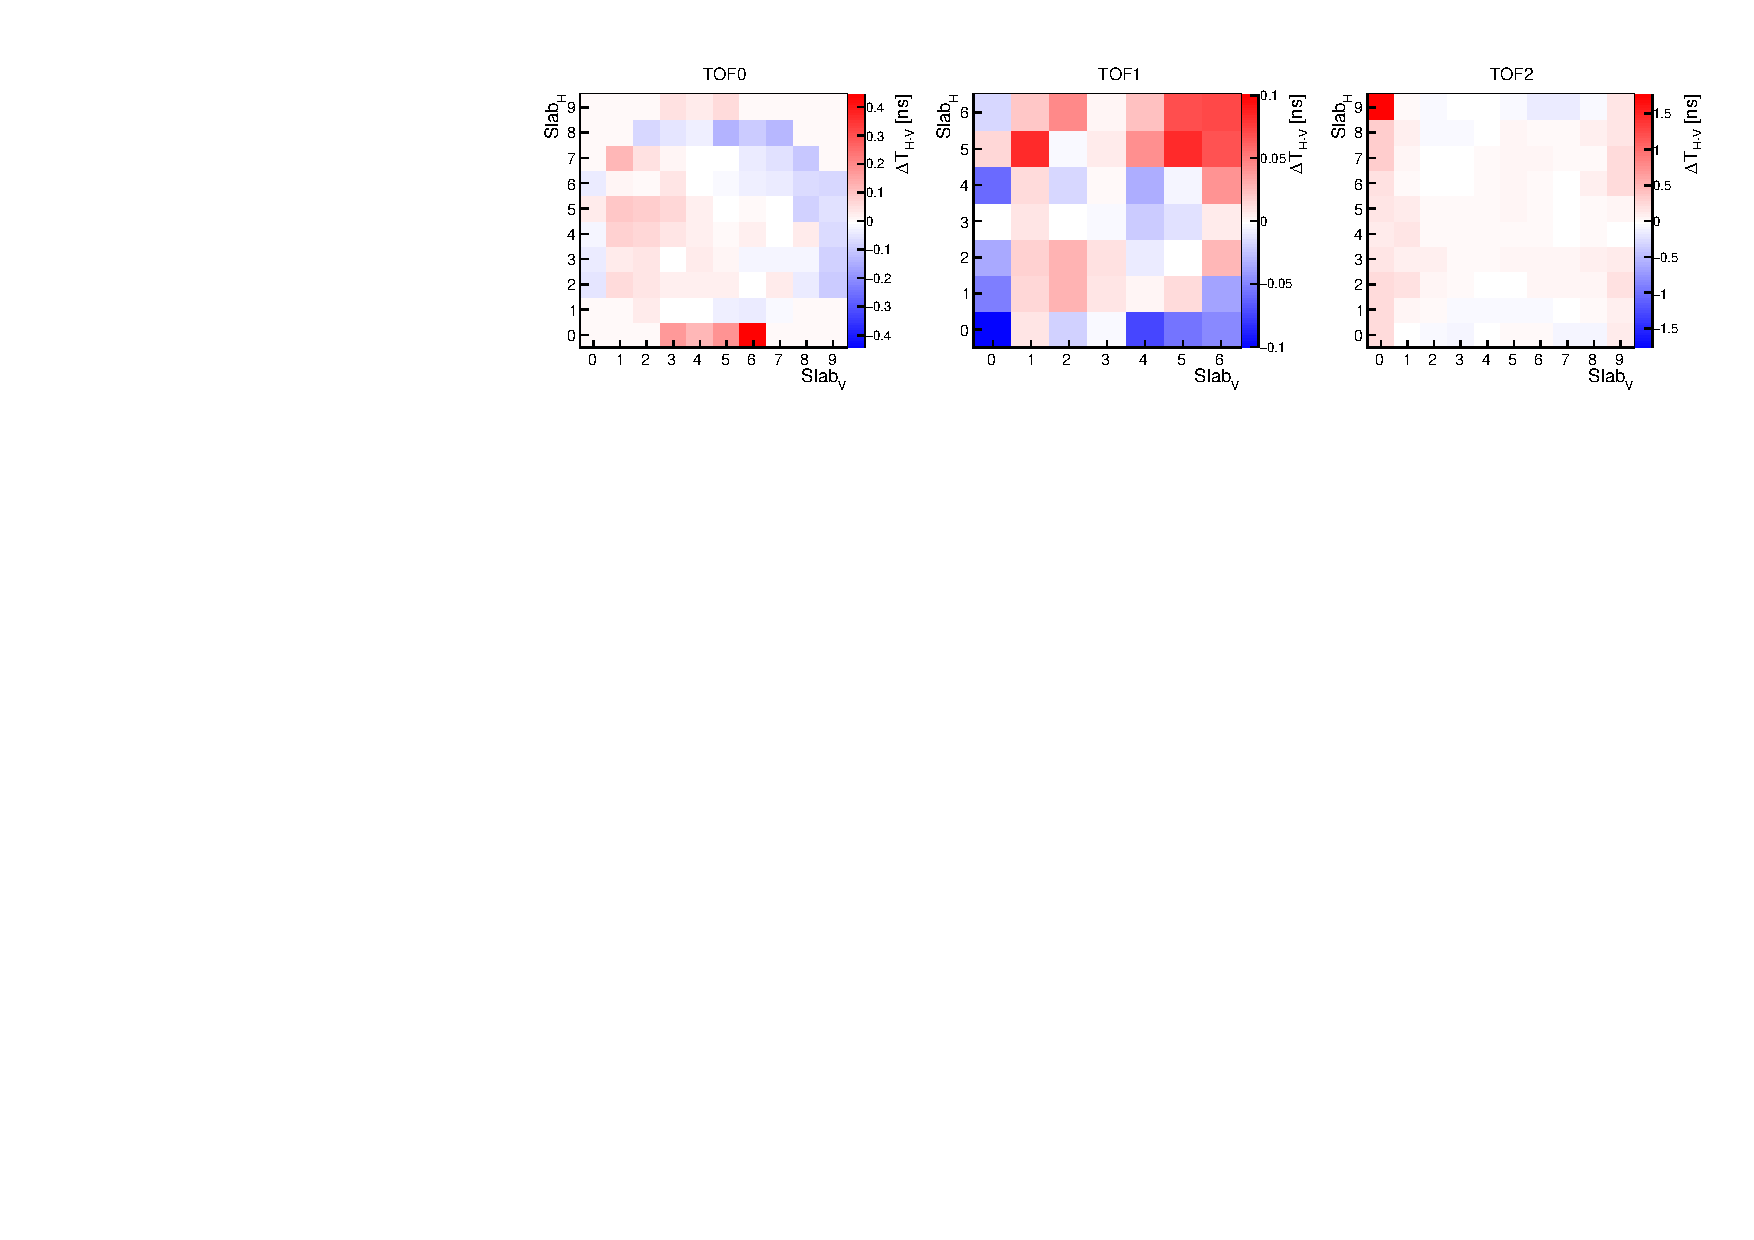
\includegraphics[width=0.9\columnwidth]{05_slab_dt_offset_by_pixel_2d} \\
  \caption{Offsets in slab \DT{} for individual pixels for all 3 stations.}
  \label{fig:SlabDToffsetByPixel}
  \end{center}
\end{figure}


\begin{figure}
  \begin{center}
  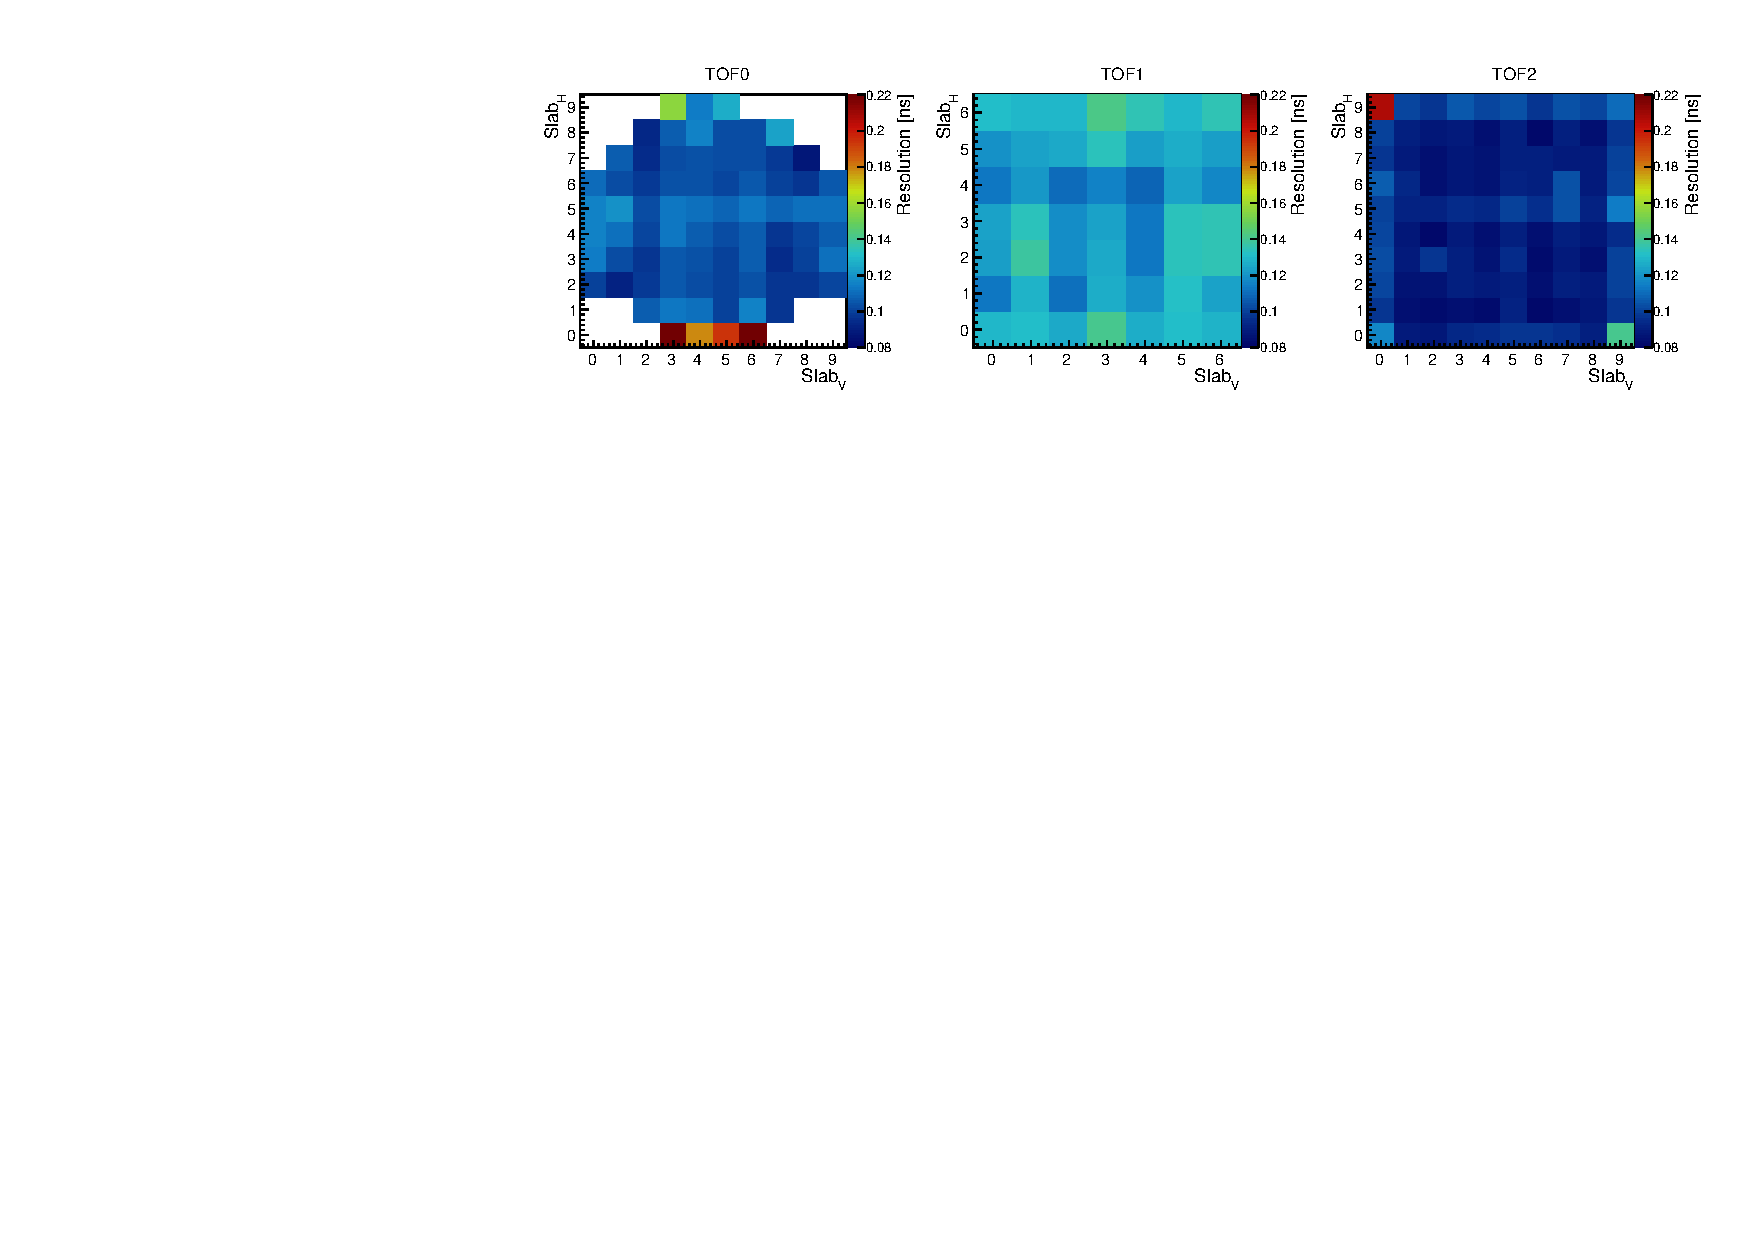
\includegraphics[width=0.9\columnwidth]{06_slab_dt_resolution_by_pixel_2d} \\
  \caption{Spread in the slab \DT{} distributions of each pixel.}
  \label{fig:SlabDTresByPixel}
  \end{center}
\end{figure}

Overall performance can be inferred from the combined slab \DT{}
distributions. The plots in Figure~\ref{fig:SlabDtAll} show that they all centre
approximately at 0~ns and they exhibit very similar resolutions, with TOF1
having the largest spread.


\begin{figure}
  \begin{center}
  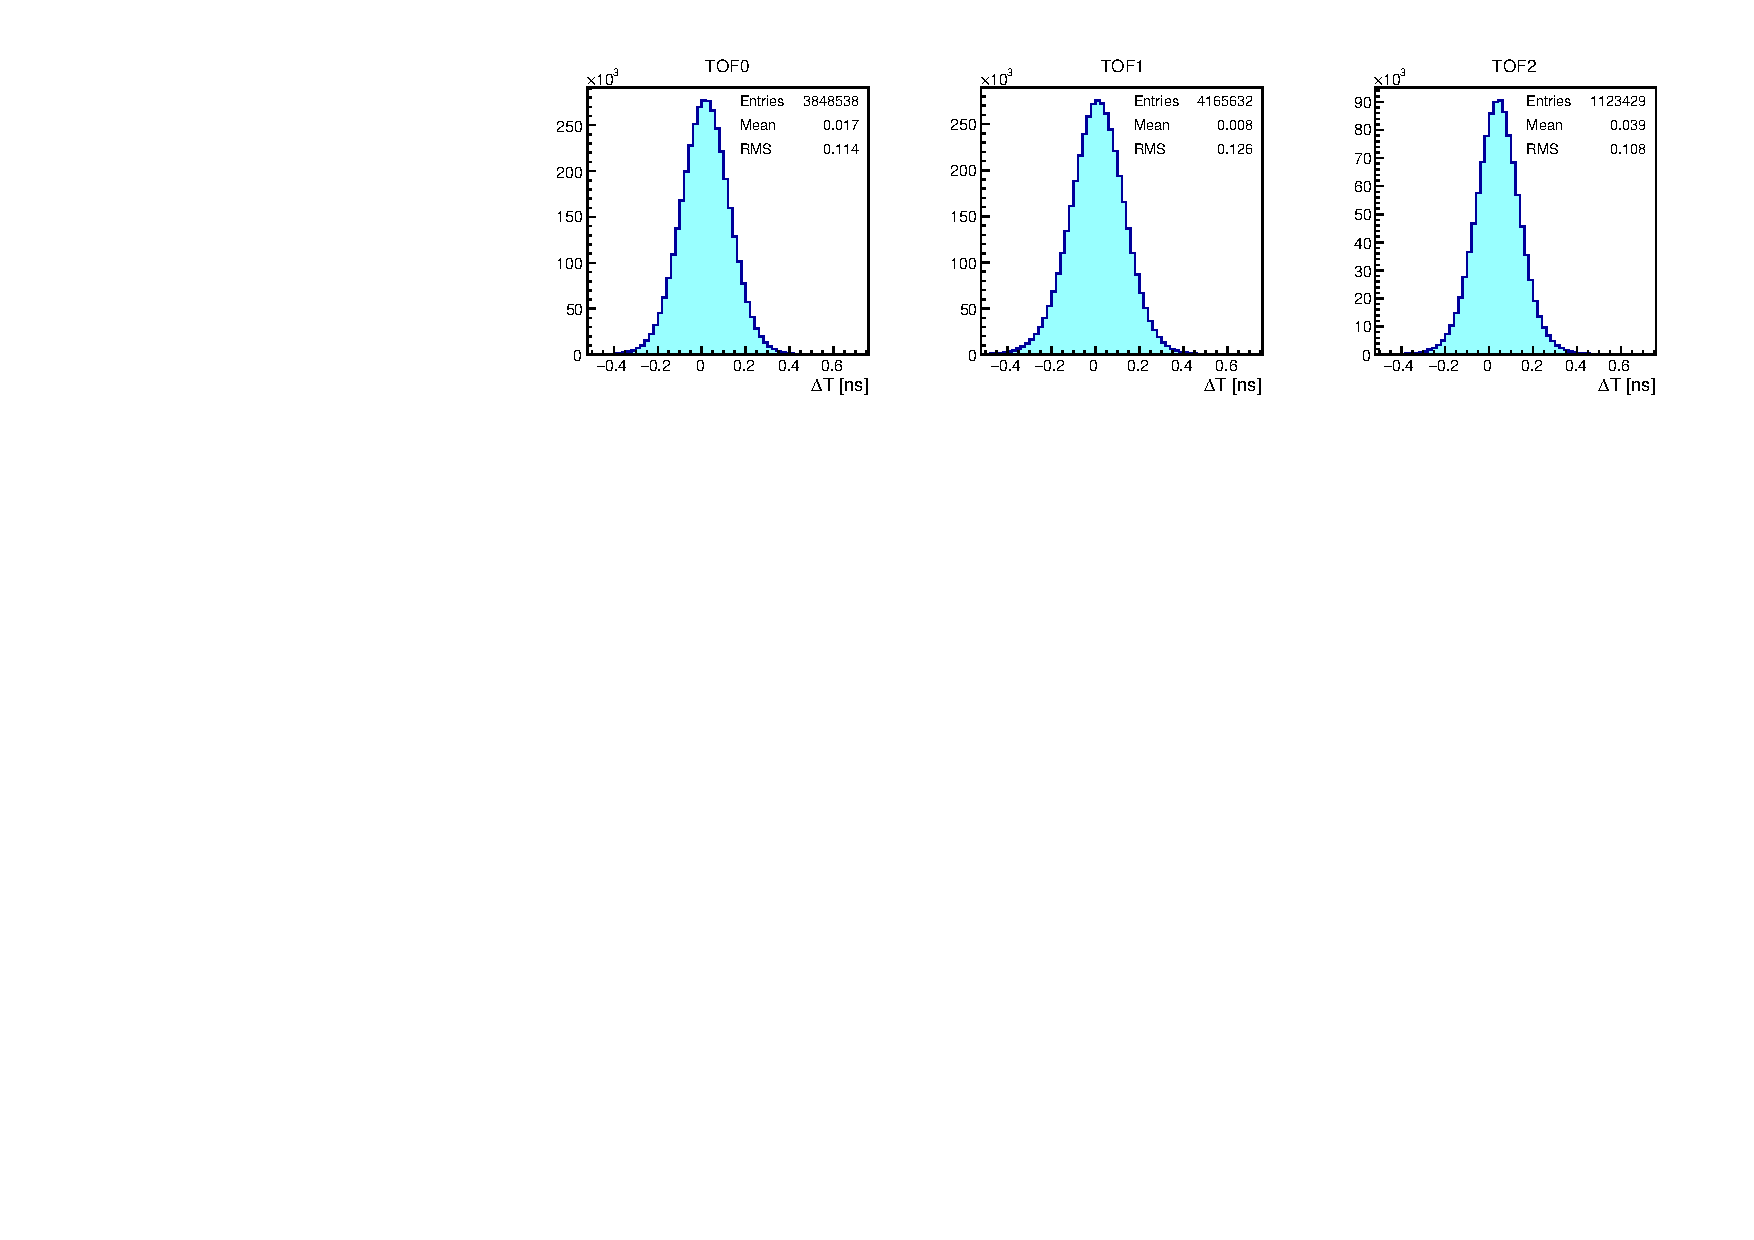
\includegraphics[width=0.9\columnwidth]{07_overall_slab_dt} \\
  \caption{Overall slab \DT{} distributions. Total width of the
    distribution is due to the resolution of individual pixels and due to
    the offsets in their \DT{} distributions.}
  \label{fig:SlabDtAll}
  \end{center}
\end{figure}

% Error of the time-of-flight measurement is a combination of intrinsic
% resolution of each TOF station and errors in the calibrations of
% individual \malert{scintillation counters}. The total error of t-o-f
% as measured by stations $i$ and $j$ is considered as:
% %
% \begin{equation}
%   \label{eq:tof:err}
%   \sigma_{\text{TOF}_{ij}} = \sqrt{ \sigma^2_{i} + \sigma^2_{j} +
%     \sigma^2_{\text{calib}} } .
% \end{equation}
% %
% Individual uncertainties $\sigma_i$ are assumed to be statistically
% uncorrelated. Error of the calibration method, $\sigma_\text{calib}$,
% consists of uncertainties correlated and uncorrelated between the
% stations.

The reconstruction of a pixel by matching of 2 slabs from different
planes of each station is dependent on the slab \DT{}. The 4~ns time
window for the matching was chosen to cover the errors of the
calibrations. Yet, there were times when there were signals in slabs
in each plane of a station, but they were never matched. These events
were mostly results of multiple particles passing through the station
and causing signal in one plane only. They would never be matched in
time as they arrived within the beam bunch time stretch of about
1~\us{}. Figure~\ref{fig:SpEffByPixel} shows fractions of events where
there were signals in two perpendicular slabs and they were
time-matched. One can see lower efficiency/fraction in the peripheral
pixels which is associated with the larger fraction of multiple
particle crossings with giving signal in one slab only.



\begin{figure}[!htb]
  \begin{center}
  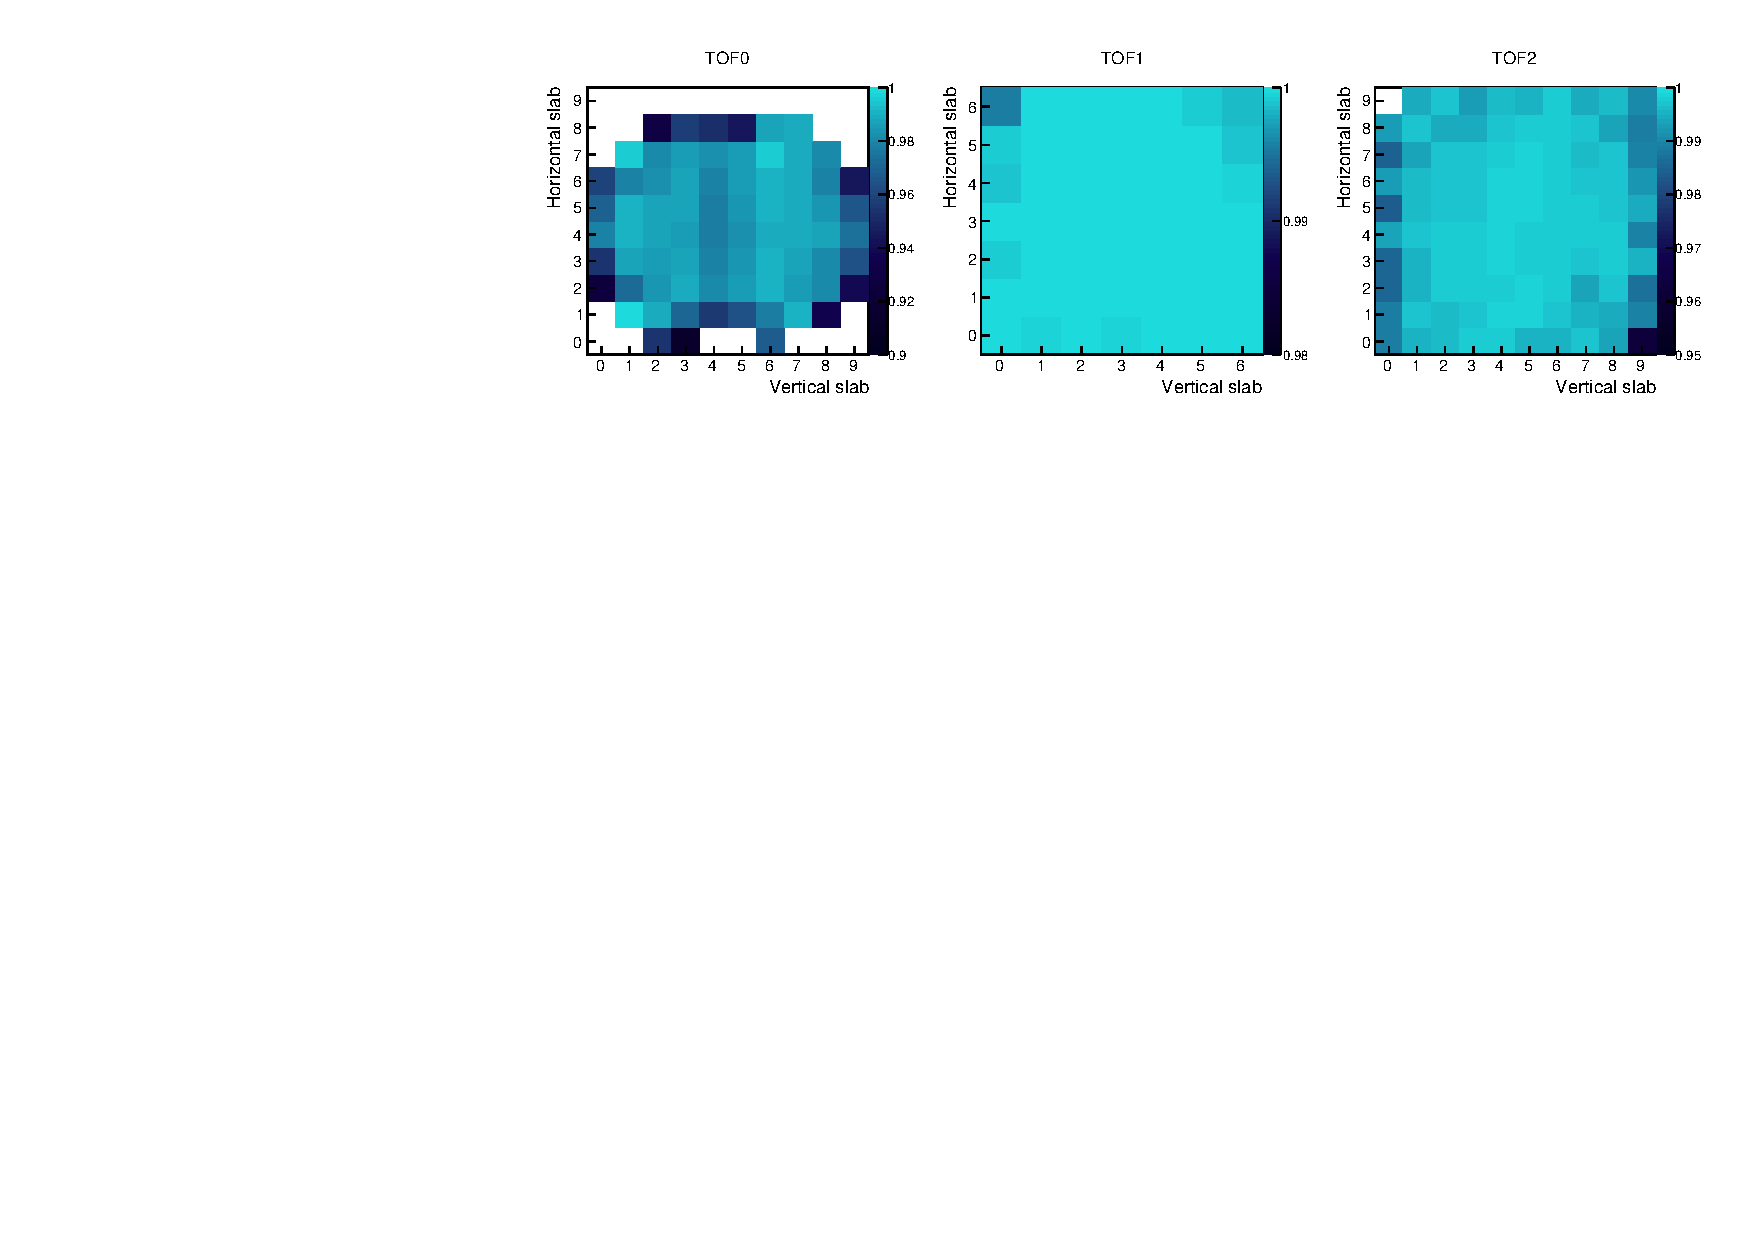
\includegraphics[width=0.9\columnwidth]{08_sp_eff_by_pixel_2d} \\
  \caption{Efficiency of space point creation if there were hits in
    two transverse slabs.}
  \label{fig:SpEffByPixel}
  \end{center}
\end{figure}


%To be changed with a better one
\begin{figure}[!htb]
  \begin{center}
    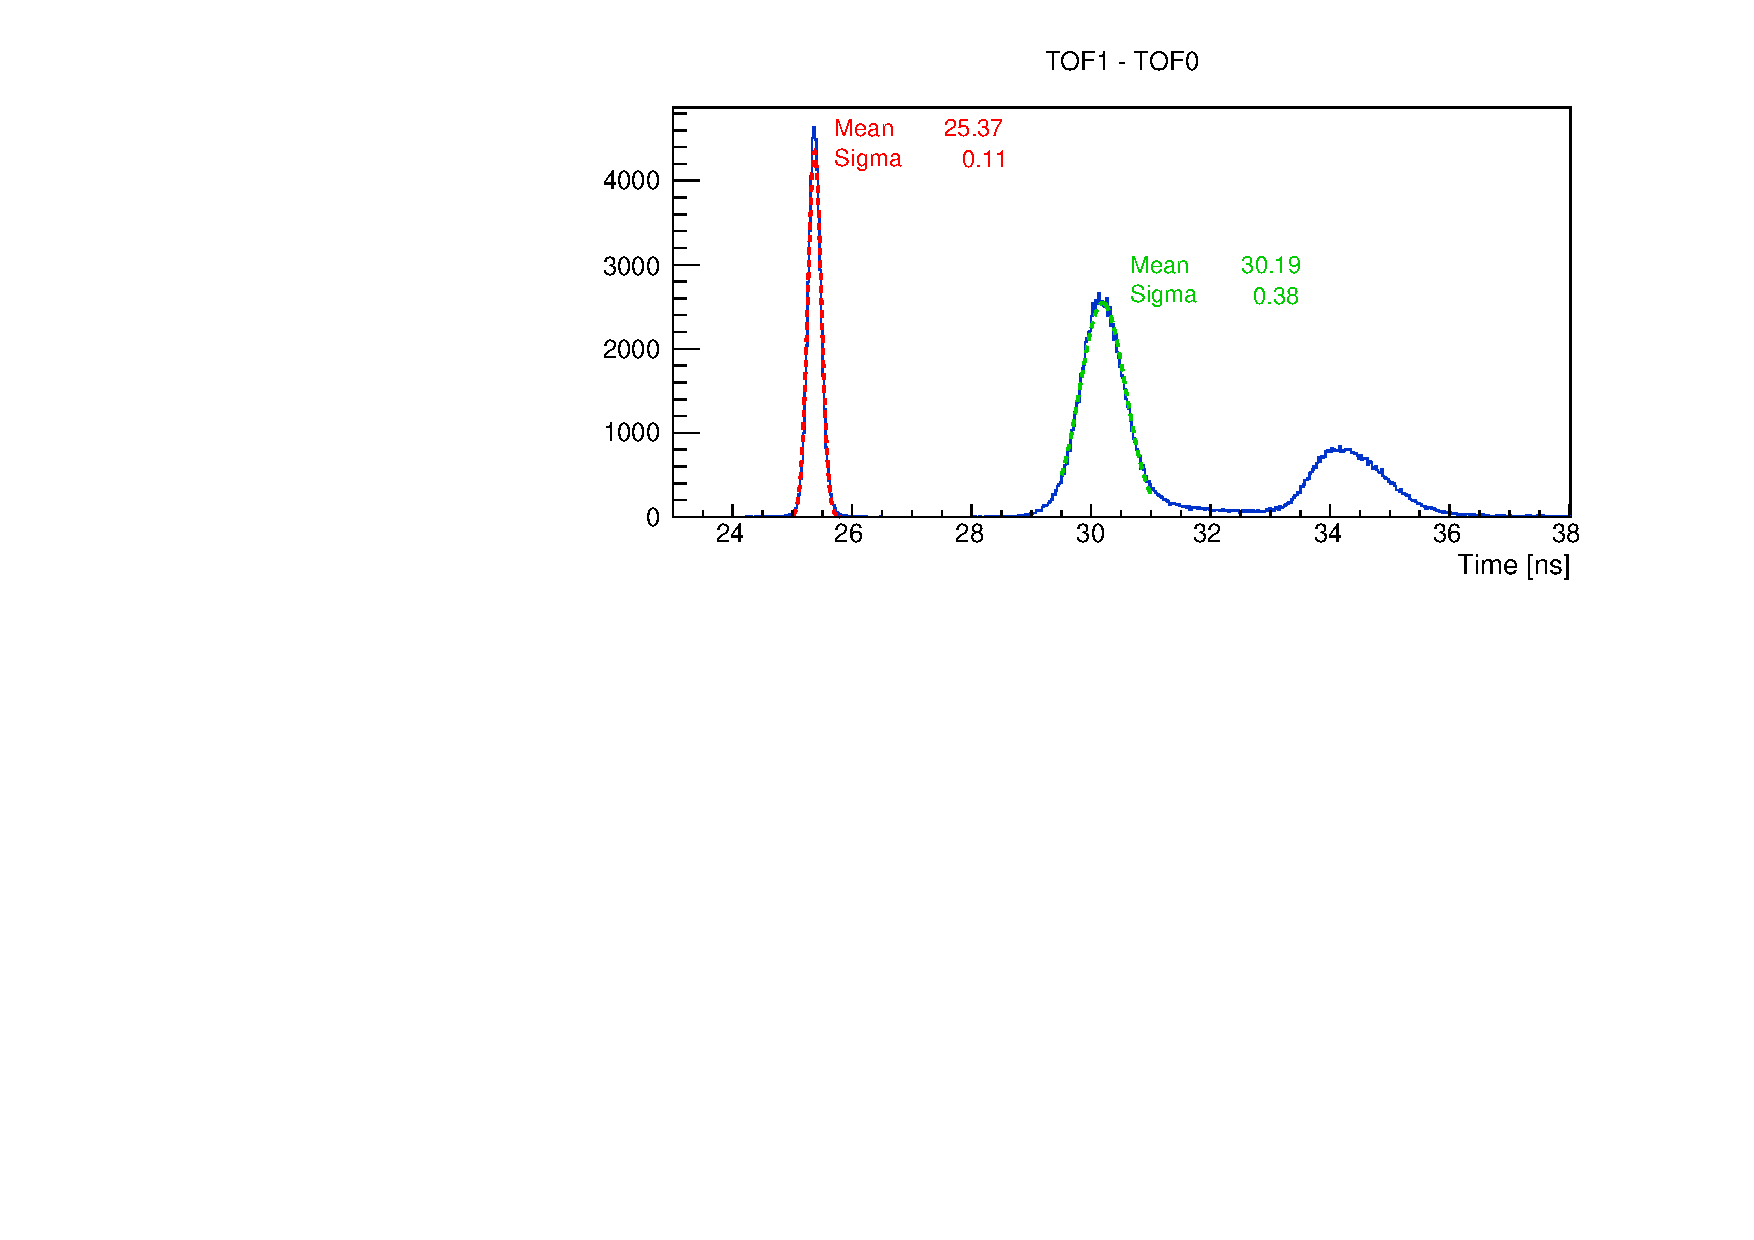
\includegraphics[width=0.6\columnwidth]{TOF_peaks.pdf}
    \caption{Time of flight between TOF0 and TOF1 for a ``pion'' beam. From the left: the well separated electron, muon and pion peaks.}
    \label{fig:TOF_peaks}
  \end{center}
\end{figure}

%%%%%%%%%%%%%%%%%%%%%%%%%%%%%%%%%%%%%%%%%%%%%%%%%%%%%%%%%%%%%%%%%%%%%%%%%%%%%%%%

% \subsubsection{Low-level Characterisation}

% \malert{maybe leave this out, likely not necessary}

% \begin{itemize}
% \item PMT charge correlation PMT0 vs PMT1 - maybe, if relevant
% \item Residual TW - this should go to the calibration section
% \item Slab DT
% \end{itemize}





% \subsubsection{Time-of-Flight Resolution and Efficiency}

% \begin{itemize}
% \end{itemize}


%%% Local Variables:
%%% mode: latex
%%% TeX-master: "../Systems-performance"
%%% End:
